% DocuFlow Class v1.1 (main.tex)
% Created by Lucas Schmirl, 2025.

% chktex-file 1 % to ignore trailing whitespace warning

\documentclass[ngerman,article,IEEE,12pt]{docuflow}

% Include definitions (titlepage setup)
% Uncomment to customize fonts:
%\usepackage{lmodern}      % Latin Modern font family
% --- Font sizes for 12pt class (default reference) ---
% \renewcommand{\tiny}{\fontsize{6}{7}\selectfont}
% \renewcommand{\scriptsize}{\fontsize{8}{9}\selectfont}
% \renewcommand{\footnotesize}{\fontsize{10}{12}\selectfont}
% \renewcommand{\small}{\fontsize{11}{13}\selectfont}
% \renewcommand{\normalsize}{\fontsize{12}{14.5}\selectfont}
% \renewcommand{\large}{\fontsize{14.4}{17}\selectfont}
% \renewcommand{\Large}{\fontsize{17.3}{20}\selectfont}
% \renewcommand{\LARGE}{\fontsize{20.7}{24}\selectfont}
% \renewcommand{\huge}{\fontsize{24.8}{29}\selectfont}
% \renewcommand{\Huge}{\fontsize{29.8}{35}\selectfont}


% --- Titlepage setup ---
\settitlebackground{PICs/title-DocuFlow.pdf}

% Titlepage content
\setTitlePageContent{
  \centering
  \vspace*{14cm}

  {\Huge\bfseries My First DocuFlow Document}\\[2ex]
  
  \vspace*{2cm}

  {\Large Author Name}\\[1ex]
  {\small \today}
}

% User-defined colors
\definecolor{FAVgreen}{RGB}{177,179,48}
\definecolor{FAVblue}{RGB}{0,142,251}
\definecolor{FAVgray}{RGB}{177,177,175}



% Macros

% ---------------- Figure macro ----------------
% Usage: \DFfigure[size]{<image path>}{<caption>}{<label>}
\newcommand{\DFfigure}[4][0.8\linewidth]{%
\begin{figure}[!htbp]
    \centering
    \includegraphics[width=#1]{#2}
    \caption{#3}\label{#4}
\end{figure}
}

% === START DOCUMENT ===
\begin{document}

% Front matter with Roman page numbering
\pagenumbering{roman}

% handle abstract, and Kurzfassung (if ngerman)
\DFmakefrontmatter

% main matter with Arabic page numbering
\pagenumbering{arabic}

% Class tutorial
% DocuFlow Class v1.0 (Tutorial)
% Created by Lucas Schmirl, 2025.

\section{Kurze Einführung in die \texttt{docuflow}-Klasse}

Die \texttt{docuflow}-Klasse ist eine LaTeX-Klasse, die speziell für wissenschaftliche Dokumentation entwickelt wurde. 
Sie bietet einige Komfortfunktionen und vorgefertigte Layouts für konsistente Formatierung.

\subsection{Aufruf der Klasse}

Die Klasse wird wie folgt eingebunden:

\begin{verbatim}
\documentclass[<Sprache>,<DokTyp>,<Zitationsstil>,<Schriftgröße>]{docuflow}
\end{verbatim}

\subsection{Mögliche Optionen}

\begin{itemize}
    \item \textbf{Sprache:} 
    \begin{itemize}
        \item \texttt{english} – Englische Lokalisierung (Standard)
        \item \texttt{ngerman} – Deutsche Lokalisierung
    \end{itemize}
    \item \textbf{Dokumenttyp:} 
    \begin{itemize}
        \item \texttt{article} – Standardartikel
        \item \texttt{report} – Berichtsmodus (Kapitel verfügbar)
        \item \texttt{book} – Buchmodus (Kapitel verfügbar)
    \end{itemize}
    \item \textbf{Zitationsstil:} 
    \begin{itemize}
        \item \texttt{apa7} – APA 7. Ausgabe
        \item \texttt{harvard} – Harvard-Stil
        \item \texttt{IEEE} – IEEE-Zitationsstil
    \end{itemize}
    \item \textbf{Schriftgröße:} 
    \begin{itemize}
        \item \texttt{10pt}, \texttt{11pt}, \texttt{12pt} – Standard-LaTeX-Schriftgrößen
    \end{itemize}
\end{itemize}

\clearpage
\subsection{Besondere Funktionen}

\begin{itemize}
    \item \textbf{Titelblatt mit Hintergrundbild:}\\
    Mit den Makros \verb|\settitlebackground{<Bildpfad>}| 
    
    und \verb|\setTitlePageContent{<Inhalt>}| kann ein individuelles Titelblatt gestaltet werden (siehe \verb|definitions.tex|).

    \item \textbf{Automatische Überschriften für Frontmatter:}\\
    Abstract, Kurzfassung und Abkürzungsverzeichnis passen sich automatisch an den Dokumenttyp an 
    
    (Artikel: \verb|\section*|, Report/Book: \verb|\chapter*|).

    \item \textbf{Bibliographie-Integration:}\\
    Biber/BibLaTeX wird direkt unterstützt. Der Stil passt sich automatisch an die Klassenoption an.

    \item \textbf{Makros für Abbildungen:}\\
    Beispiel: \verb|\DFfigure[<Breite>]{<Bild>}{<Beschriftung>}{<Label>}|
    
    \item \textbf{Deutsche Lokalisierung:}\\
    Überschriften für Abbildungsverzeichnis, Tabellenverzeichnis, Inhaltsverzeichnis und Abkürzungsverzeichnis werden automatisch gesetzt, 
    wenn \texttt{ngerman} gewählt wird (können in \verb|docuflow.cls| abgeändert werden).
\end{itemize}


\clearpage

\subsection{Aufbau der Dokumentdateien}

Die \texttt{docuflow}-Klasse ist so konzipiert, dass der Inhalt modular in mehreren 
\texttt{.tex}-Dateien organisiert wird. Jede Datei hat einen eigenen Zweck und kann unabhängig 
bearbeitet werden. Danach werden die Dateien einfach in das Hauptdokument eingebunden.

\begin{itemize}
    \item \textbf{definitions.tex:}  
    Enthält alle globalen Definitionen, Farben, Größen und Makros (z. B. für Abbildungen). 
    Diese Datei wird einmalig in \texttt{main.tex} geladen.

    \item \textbf{abstract.tex:}  
    Enthält den englischen Abstract des Dokuments. 
    Einfach den Text und Keywords bearbeiten.

    \item \textbf{kurzfassung.tex:}  
    Enthält die deutsche Kurzfassung. Diese Datei wird nur eingebunden, wenn die Klasse mit 
    \texttt{ngerman} aufgerufen wird. Analog zu \verb|abstract.tex| den Text und Keywords bearbeiten.

    \item \textbf{content.tex:}  
    Der Hauptinhalt des Dokuments. Alle Kapitel, Abschnitte oder sonstiger Text wird hier eingefügt.  

    \item \textbf{bibliography.bib:}  
    Enthält alle Literaturangaben im BibLaTeX-Format. 
    
    Sie wird über \verb|\addbibresource{bibliography.bib}| in der Klasse eingebunden.

    \item \textbf{PICs/\textless name\textgreater.pdf/png/jpg:}  
    Dieser Ordner enthält alle Grafiken, die über \verb|\DFfigure| oder manuell eingefügt werden.
\end{itemize}

\noindent
Hintergrund für diese Struktur ist, dass jede Datei separat bearbeitet wird, 
ohne das Hauptdokument zu verändern. Das Hauptdokument \texttt{main.tex} bindet 
alle Dokumente ein und sorgt für die korrekte Reihenfolge.\\

Alle weiteren, in diesem Ordner enthaltenen, Dokumente:

\begin{itemize}[noitemsep]
    \item \verb|luaLatexFontDemo.tex| 
    \item \verb|pdfLatexFontDemo.tex| 
    \item \verb|tutorial.tex| 
    \item \verb|snippets.tex|
\end{itemize}

dienen der Demonstration und sind nicht notwendig für die Funktion der Klasse 
(können in \verb|main.tex| auskommentiert werden).


\clearpage

\subsection{Beispiel für die Verwendung}

In \verb|definitions.tex|:

\begin{verbatim}
    \renewcommand{\title}{My First DocuFlow Document}
    \renewcommand{\author}{Lucas Schmirl, MSc.}
    \settitlebackground{PICs/title-DocuFlow.pdf}
    \setTitlePageContent{
    \begin{center}
        \title\\
        \author\\
        \today
    \end{center}}
\end{verbatim}

\noindent In \verb|main.tex|:

\begin{verbatim}
    \documentclass[ngerman,article,IEEE,12pt]{docuflow}
    % Uncomment to customize fonts:
%\usepackage{lmodern}      % Latin Modern font family
% --- Font sizes for 12pt class (default reference) ---
% \renewcommand{\tiny}{\fontsize{6}{7}\selectfont}
% \renewcommand{\scriptsize}{\fontsize{8}{9}\selectfont}
% \renewcommand{\footnotesize}{\fontsize{10}{12}\selectfont}
% \renewcommand{\small}{\fontsize{11}{13}\selectfont}
% \renewcommand{\normalsize}{\fontsize{12}{14.5}\selectfont}
% \renewcommand{\large}{\fontsize{14.4}{17}\selectfont}
% \renewcommand{\Large}{\fontsize{17.3}{20}\selectfont}
% \renewcommand{\LARGE}{\fontsize{20.7}{24}\selectfont}
% \renewcommand{\huge}{\fontsize{24.8}{29}\selectfont}
% \renewcommand{\Huge}{\fontsize{29.8}{35}\selectfont}


% --- Titlepage setup ---
\settitlebackground{PICs/title-DocuFlow.pdf}

% Titlepage content
\setTitlePageContent{
  \centering
  \vspace*{14cm}

  {\Huge\bfseries My First DocuFlow Document}\\[2ex]
  
  \vspace*{2cm}

  {\Large Author Name}\\[1ex]
  {\small \today}
}

% User-defined colors
\definecolor{FAVgreen}{RGB}{177,179,48}
\definecolor{FAVblue}{RGB}{0,142,251}
\definecolor{FAVgray}{RGB}{177,177,175}



% Macros

% ---------------- Figure macro ----------------
% Usage: \DFfigure[size]{<image path>}{<caption>}{<label>}
\newcommand{\DFfigure}[4][0.8\linewidth]{%
\begin{figure}[!htbp]
    \centering
    \includegraphics[width=#1]{#2}
    \caption{#3}\label{#4}
\end{figure}
}
    \begin{document}
        \pagenumbering{roman}
        \DFmakefrontmatter
        \pagenumbering{arabic}
        % DocuFlow Class v1.0 (content.tex)
% Created by Lucas Schmirl, 2025.

\section{Einführung (\texttt{snippets})}
Hier steht der hauptsächliche \glqq~Inhalt\grqq des Dokuments.

Verwende das figure-macro der Klasse um Bilder einzufügen:
\DFfigure[0.6\linewidth, angle=-90]{PICs/hund}{Das ist ein Hund.}{fig:smallFigure}

Abkürzungen wie diese:
\ac{CPU}, \ac{RAM}, and \ac{GPU}, 
können nach der Definition in \texttt{acronym} in \texttt{main.tex} verwendet werden.


    \subsection{Überschrift 2. Ebene}
    Zitate können mit: \parencite{knuth1984} oder~\cite{knuth1984} gesetzt werden.

    Farbige  \textcolor{FAVblue}{Texte} funktionieren so.
        \printbibliography[title=\bibname, heading=bibintoc]
        \addcontentsline{toc}{section}{\listfigurename}
        \listoffigures
        \addcontentsline{toc}{section}{\listtablename}
        \listoftables
        \addcontentsline{toc}{section}{\lstlistlistingname}
        \lstlistoflistings
        \addcontentsline{toc}{section}{\acronymname}
        \DFabstractSection{\acronymname}
        \begin{acronym}[AFT]
        \acro{AFT}{Acronym for testing}
        \end{acronym}
        \appendix
        \DFautoSection{\appendixname~A}
    \end{document}

\end{verbatim}

\clearpage

\subsection{Kompilieren des Dokuments}\label{settingsjson}

Um das Dokument zu kompilieren, verwenden Sie einen LaTeX-Editor wie TeXstudio oder Visual Studio Code mit der LaTeX-Workshop-Erweiterung. 
Bei der Verwendung von Visual Studio Code stellen Sie sicher, dass die \verb|settings.json| (User Settings, erreichbar mit F1 + settings.json) korrekt konfiguriert ist (siehe \verb|README.md|).\\

\textbf{Achtung}, der Block im \verb|README.md| ist nur ein Ausschnitt der gesamten \verb|settings.json| Datei. 
Falls Sie schon eine bestehende \verb|settings.json| haben, fügen Sie den Block innerhalb der geschwungenen Klammern ein.
Falls Sie keine \verb|settings.json| haben, können Sie eine neue anlegen und den gesamten Inhalt einfügen. 
Der Block muss sich jedenfalls innerhalb geschweifter Klammern befinden.\\

\noindent\verb|settings.json:|
\begin{verbatim}
{
        some other settings,
        // LaTeX Settings
        // LaTeX Tools
        // LaTeX Recipes
}
\end{verbatim}
\clearpage

% Main content
% DocuFlow Class v1.0 (content.tex)
% Created by Lucas Schmirl, 2025.

\section{Einführung (\texttt{snippets})}
Hier steht der hauptsächliche \glqq~Inhalt\grqq des Dokuments.

Verwende das figure-macro der Klasse um Bilder einzufügen:
\DFfigure[0.6\linewidth, angle=-90]{PICs/hund}{Das ist ein Hund.}{fig:smallFigure}

Abkürzungen wie diese:
\ac{CPU}, \ac{RAM}, and \ac{GPU}, 
können nach der Definition in \texttt{acronym} in \texttt{main.tex} verwendet werden.


    \subsection{Überschrift 2. Ebene}
    Zitate können mit: \parencite{knuth1984} oder~\cite{knuth1984} gesetzt werden.

    Farbige  \textcolor{FAVblue}{Texte} funktionieren so.
\clearpage

% Example snippets
% DocuFlow Class v1.0 (Snippets)
% Created by Lucas Schmirl, 2025.

\section{Allgemeine \LaTeX Beispiele}

Querverweise werden in \LaTeX{} automatisch erzeugt und verwaltet, damit sie leicht aktualisiert werden können.
Beispiele sind~\cite{Ko05a},~\cite{Ko05b},~\cite{MiGo05},~\cite{TeGo14},~\cite{HuHa07}.
Es wird dringend empfohlen, Biber oder BibTeX zu verwenden (wie in diesen Beispielen).
Die Quellen werden in \verb|bibliography.bib| definiert, (Templates verfügbar).\\

Abkürzungen wie die folgenden sind im Abkürzungsverzeichnis vermerkt:
\ac{CPU}, \ac{RAM}, und \ac{GPU}. Diese können nach der Definition in \texttt{acronym} in \texttt{main.tex} verwendet werden.\\

Eine \glqq{}schöne\grqq{} Farbe ist \textcolor{FAVgreen}{dieses Grün (RGB:~177,179,48)}.\\

\noindent Wenn ein neuer Absatz \textcolor{red}{nicht} eingerückt werden soll funktioniert das so.\\

Anführungszeichen können auf \glq{}diese\grq{}, 'diese' und \glqq{}jene\grqq{} Weise verwendet werden.\\

So macht man einen Zeilenumbruch.\\
Und so einen Seitenumbruch.\clearpage

    
    \subsection{Abbildungen}

        \begin{figure}[!htbp]
            \centering
            \includegraphics[width=0.5\linewidth]{PICs/hund.png}
            \caption{Das ist ein Hund.}
            \label{Abb:hund}
        \end{figure}

        Für das Einfügen von Bildern kann auch das \verb|figure-macro| der Klasse verwendet werden.
        
        \DFfigure[0.5\linewidth, angle=-90]{PICs/hund}{Der selbe Hund (rotiert).}{fig:smallFigure}


    \clearpage
    \subsection{Tabellen}

        \begin{table}[!htbp]
                \centering
                \begin{tabular}{| p{0.3\linewidth} | p{0.3\linewidth} | p{0.3\linewidth} |}\hline
                %\begin{tabular}{| c | l | r |}\hline
                Datum & Produktionsschritt & Abteilung\\\hline
                15.02.2025 & Rohstoffmischung & Chemielabor\\
                17.02.2025 & Qualitätsprüfung & Labor\\
                20.02.2025 & Abfüllung & Produktion\\
                22.02.2025 & Verpackung & Logistik\\\hline
                \end{tabular}
                \caption{Produktionsplan für Reinigungsmittel \glqq{}EcoClean\grqq{}.}\label{tab:1}
            \end{table}


    \subsection{Verweise, Links}
        Das ist ein Verweis auf Tabelle~\ref{tab:1}. Das gezeigte Tabellenformat ist nur ein Beispiel.
        Tabellen können individuell gestaltet werden, dazu gerne auch mal dieses \hyperref{https://www.tablesgenerator.com/}{category}{name}{Tool} austesten.\\

        Hier wird zum Beispiel auf Abbildung~\ref{Abb:hund} verwiesen.\\


    \subsection{Mathematische Formeln}
    Im nächsten Unterkapitel werden Formeln wie z.B. Formel~\ref{Gl:1} dargestellt.
    Griechische Buschtaben können auf diese weise eingefügt werden: 
    $\alpha, \beta, \gamma, \rho, \sigma, \delta, \epsilon$.

        \begin{align}
            x &= -\frac{p}{2}\pm\sqrt{\frac{p^2}{4}-q}\label{Gl:1}\\
            e^{i \pi} + 1 &= 0\label{Gl:2}\\
            C &= \sum_{n=-\infty}^{+\infty} f(\frac{\partial x}{\partial y}w)
        \end{align}


    \clearpage
    \subsection{Code}

    Code kann mithilfe des Pakets \verb|listing| dargestellt werden.
        \begin{lstlisting}[language=C++,name={C++ Beispiel},label={sc:bsp:1}]
            #include <iostream>

            void SayHello(void)
            {
                // Kommentar
                cout << "Hello World!" << endl;
            }

            int main(int argc, char **argv)
            {
                SayHello();
                return 0;
            }
            \end{lstlisting}

    \subsection{Grafiken (Zeichnen)}
    % This is how to draw manually
    \begin{figure}[!htbp]
        \centering
        \begin{tikzpicture}
            \node[draw=orange, fill=orange!20] (a) {\large A};
            \node[draw=yellow, fill=yellow!20, right= of a] (b) {\Large B};
            \node[circle, draw=green, fill=green!20, right= of b] (c) {\Large C};
            \draw[->] (a) -- (b);
            \draw[->>] (b) -- (c);
        \end{tikzpicture}\caption{Selbst gezeichnete Grafik: \hyperref{https://greysonwesley.com/files/TikZCheatsheet.pdf}{}{}{Cheatsheet}}\label{fig:my_graph}
    \end{figure}
    
    % This is how to draw manually (by Gii)
    \begin{figure}[!htbp]
        \centering
        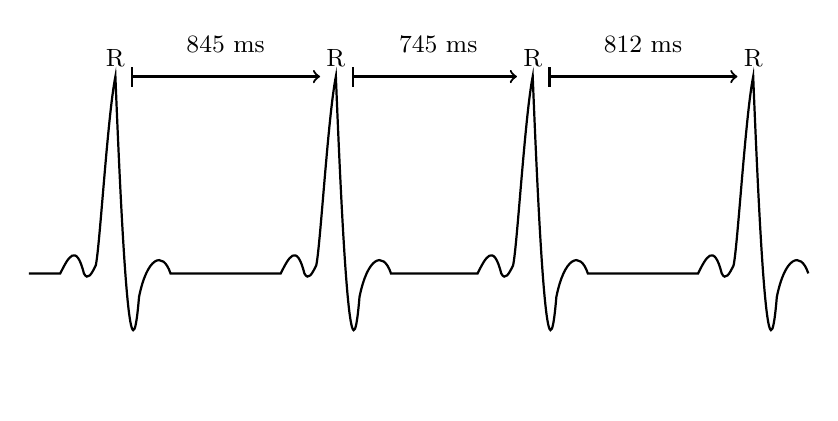
\begin{tikzpicture}[scale=1, every node/.style={font=\small}]
            % EKG-Tracing mit variierenden Abständen
            \draw[thick]
            (0,0) -- (0.4,0)
            .. controls (0.5,0.2) and (0.6,0.4) .. (0.7,0)
            .. controls (0.75,-0.1) and (0.8,0) .. (0.85,0.1)
            .. controls (0.9,0.3) and (1,2) .. (1.1,2.5)
            .. controls (1.2,0) and (1.3,-1.5) .. (1.4,-0.3)
            .. controls (1.5,0.2) and (1.7,0.3) .. (1.8,0)
            -- (3.2,0)
            .. controls (3.3,0.2) and (3.4,0.4) .. (3.5,0)
            .. controls (3.55,-0.1) and (3.6,0) .. (3.65,0.1)
            .. controls (3.7,0.3) and (3.8,2) .. (3.9,2.5)
            .. controls (4.0,0) and (4.1,-1.5) .. (4.2,-0.3)
            .. controls (4.3,0.2) and (4.5,0.3) .. (4.6,0)
            -- (5.7,0)
            .. controls (5.8,0.2) and (5.9,0.4) .. (6.0,0)
            .. controls (6.05,-0.1) and (6.1,0) .. (6.15,0.1)
            .. controls (6.2,0.3) and (6.3,2) .. (6.4,2.5)
            .. controls (6.5,0) and (6.6,-1.5) .. (6.7,-0.3)
            .. controls (6.8,0.2) and (7.0,0.3) .. (7.1,0)
            -- (8.5,0)
            .. controls (8.6,0.2) and (8.7,0.4) .. (8.8,0)
            .. controls (8.85,-0.1) and (8.9,0) .. (8.95,0.1)
            .. controls (9.0,0.3) and (9.1,2) .. (9.2,2.5)
            .. controls (9.3,0) and (9.4,-1.5) .. (9.5,-0.3)
            .. controls (9.6,0.2) and (9.8,0.3) .. (9.9,0);
            
            % R-Markierungen bei Peaks
            \node[above] at (1.1,2.5) {R};
            \node[above] at (3.9,2.5) {R};
            \node[above] at (6.4,2.5) {R};
            \node[above] at (9.2,2.5) {R};
            
            % Pfeile, horizontal auf Höhe der R, Start/Ende weiter entfernt
            \draw[|->, thick] (1.3,2.5) -- (3.7,2.5);
            \node[above=5pt] at (2.5,2.5) {845 ms};
            
            \draw[|->, thick] (4.1,2.5) -- (6.2,2.5);
            \node[above=5pt] at (5.2,2.5) {745 ms};
            
            \draw[|->, thick] (6.6,2.5) -- (9.0,2.5);
            \node[above=5pt] at (7.8,2.5) {812 ms};
        \end{tikzpicture}
        \caption{Schematische Darstellung eines EKG-Signals mit RR-Intervallen.}
        \label{fig:puls}
	\end{figure}

    % This file was created with a plot in python using tikzmaker (https://tikzmaker.com/editor)
    \begin{figure}[!ht]
        \centering
        \resizebox{0.7\textwidth}{!}{
        \begin{circuitikz}
        \tikzstyle{every node}=[font=\LARGE]
            \draw (7.5,13.25) to[american voltage source,l={ \small 5V 100mA}] (9.5,13.25);
            \draw (9.5,13.25) to[rmeter, t=V,l={ \small 3.4V}] (13.5,13.25);
            \draw [ fill={rgb,255:red,197; green,255; blue,71} ](13.5,13.25) to[lamp] (13.5,11.5);
            \draw (7.5,11.5) to[R,l={ \small 1k$\Omega$}] (10.75,11.5);
            \draw [short] (7.5,13.25) -- (7.5,11.5);
            \draw [short] (10.75,11.5) .. controls (12.25,11.5) and (12.25,11.5) .. (13.5,11.5);
        \end{circuitikz}}\caption{Erstellt mithilfe von \hyperref{https://tikzmaker.com/editor}{category}{name}{tikzmaker}.}\label{fig:tikzmaker}
    \end{figure}
    
    % This file was created with a plot in python using tikzplotlib v0.10.1. (https://pypi.org/project/tikzplotlib/)
    \begin{figure}\centering
        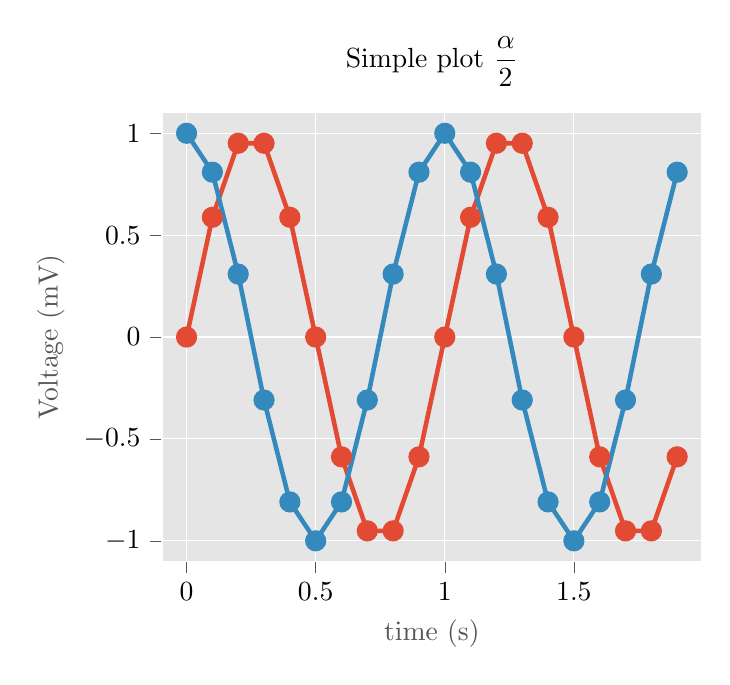
\begin{tikzpicture}
            \definecolor{chocolate2267451}{RGB}{226,74,51}
            \definecolor{dimgray85}{RGB}{85,85,85}
            \definecolor{gainsboro229}{RGB}{229,229,229}
            \definecolor{steelblue52138189}{RGB}{52,138,189}
            \begin{axis}[
                axis background/.style={fill=gainsboro229},
                axis line style={white},
                tick align=outside,
                tick pos=left,
                title={Simple plot \(\displaystyle \frac{\alpha}{2}\)},
                x grid style={white},
                xlabel=\textcolor{dimgray85}{time (s)},
                xmajorgrids,
                xmin=-0.095, xmax=1.995,
                xtick style={color=dimgray85},
                y grid style={white},
                ylabel=\textcolor{dimgray85}{Voltage (mV)},
                ymajorgrids,
                ymin=-1.1, ymax=1.1,
                ytick style={color=dimgray85}
                ]
                \addplot [line width=1.64pt, chocolate2267451, mark=*, mark size=3, mark options={solid}]
                table {%
                0 0
                0.1 0.587785252292473
                0.2 0.951056516295154
                0.3 0.951056516295154
                0.4 0.587785252292473
                0.5 1.22464679914735e-16
                0.6 -0.587785252292473
                0.7 -0.951056516295154
                0.8 -0.951056516295154
                0.9 -0.587785252292473
                1 -2.44929359829471e-16
                1.1 0.587785252292474
                1.2 0.951056516295154
                1.3 0.951056516295154
                1.4 0.587785252292473
                1.5 3.67394039744206e-16
                1.6 -0.587785252292473
                1.7 -0.951056516295154
                1.8 -0.951056516295154
                1.9 -0.587785252292473
                };
                \addplot [line width=1.64pt, steelblue52138189, mark=*, mark size=3, mark options={solid}]
                table {%
                0 1
                0.1 0.809016994374947
                0.2 0.309016994374947
                0.3 -0.309016994374948
                0.4 -0.809016994374947
                0.5 -1
                0.6 -0.809016994374947
                0.7 -0.309016994374948
                0.8 0.309016994374947
                0.9 0.809016994374947
                1 1
                1.1 0.809016994374947
                1.2 0.309016994374947
                1.3 -0.309016994374947
                1.4 -0.809016994374947
                1.5 -1
                1.6 -0.809016994374948
                1.7 -0.309016994374946
                1.8 0.309016994374947
                1.9 0.809016994374947
                };
            \end{axis}
        \end{tikzpicture}\caption{Erstellt mithilfe von \hyperref{https://pypi.org/project/tikzplotlib/}{category}{name}{Python tikzplotlib}.}\label{fig:tikzplotlib}
    \end{figure}
    \clearpage

% Print bibliography
%\addcontentsline{toc}{section}{\bibname}
\printbibliography[title=\bibname, heading=bibintoc]
\clearpage

% Print list of figures
\addcontentsline{toc}{section}{\listfigurename}
\listoffigures
\clearpage

% Print list of tables
\addcontentsline{toc}{section}{\listtablename}
\listoftables
\clearpage

% Print list of codes
\addcontentsline{toc}{section}{\lstlistlistingname}
\lstlistoflistings
\clearpage

% Print acronyms
\addcontentsline{toc}{section}{\acronymname}
\DFabstractSection{\acronymname}
\begin{acronym}[RAM]  % widest acronym for spacing
  \acro{CPU}{Central Processing Unit}
  \acro{RAM}{Random Access Memory}
  \acro{GPU}{Graphics Processing Unit}
  \acro{TBD}{The best dog}
\end{acronym}
\clearpage

%
% Hier beginnt der Anhang.
%
\clearpage
\appendix
\DFautoSection{\appendixname~A}
\clearpage
\DFautoSection{\appendixname~B}


\end{document}
